\documentclass[final,leqno,onefignum,onetabnum]{siamltexmm}

\usepackage{amsmath}
\usepackage{cleveref}

\title{Implementation of a lattice Boltzmann method for immiscible two-phase flow simulations using the level set method} 

\author
{Lorenz Hufnagel, Daniel Zint\\
Chair for System-Simulation, Friedrich Alexander Univerit\"at Erlangen-N\"urnberg\\
Cauerstr. 11, 91058 Erlangen, Germany\\
lorenz.hufnagel@fau.de, daniel.zint@fau.de % ist das so richtig?
}

\begin{document}
\maketitle
\newcommand{\slugmaster}{%
\slugger{}{}{}{}{}}%slugger should be set to juq, siads, sifin, or siims

\begin{abstract}
	We implemented the lattice Boltzmann method for immiscible multiphase flow simulations and combined it with the level set method according to the paper of G. Th\"ommes et al. \cite{Thoemmes}. The level set method is used to compute the movement of the interface between the two phases. The input for the level set method is computed by the lattice Boltzmann method. We verified our implementation with different test cases.
\end{abstract}

\begin{keywords}
	Lattice Boltzmann method,
	Level set method,
	Two-phase,
	Multiphase
\end{keywords}

%\begin{AMS}\end{AMS}


\pagestyle{myheadings}
\thispagestyle{plain}
%\markboth{TEX PRODUCTION}{USING SIAM'S MM \LaTeX\ MACROS}

\section{Introduction}
In engineering the immiscible multiphase flow problem often needs to be considered. For example, bubble dynamics are decisive for the design of chemical reactors \cite{trygg}. Also, fingering in oil recovery is a common multiphase problem.

In the following we will restrict ourselves to two fluid phases, but the procedure is also applicable for multiple phases. 
There are different approaches to solve the immiscible two-phase problem. The most spread among these is the colour gradient method of Gunstensen and Rothman \cite{GRcg1,GRcg2,GRcg3}. The downside of this method is that it is only applicable for small density and viscosity differences. Another approach is the concept of {\it interaction potentials} by Shan and Chen \cite{ShanChen1,ShanChen2}. This method actually models miscible fluids and can only approximately describe the behavior of immiscible fluids. Furthermore, there are free surface methods which only take one fluid into account for computation \cite{Koerner,Scardovelli,Hirt}. They work best for large viscosity and density ratios.

In this publication we use a hybrid lattice Boltzmann level set method. The motion of the interface is modeled by the level set method. The input data for the level set method is given by the lattice Boltzmann method (LBM), which is applied independently for each fluid. This method has the advantage that it allows large ranges of viscosity- and density-ratios between the fluid phases, while describing a sharp interface.

The incompressible two-phase flow problem can be described mathematically with the Navier-Stokes equations for two incompressible fluids \cref{nse1,nse2}, see \cite{ferziger}. To apply them, we distribute our domain into three parts: $\Omega_1$ and $\Omega_2$ describe the two fluids and $\Gamma = \delta\Omega_1 \cap \delta\Omega_2$ is the interface in-between (\cref{intro_phases}). The material properties in each fluid are constant and the interface is assumed to be sharp. Thus, the overall material properties are discontinuous and the fluids will not mix.
\begin{figure}[h!]
	\flushright
	\hfill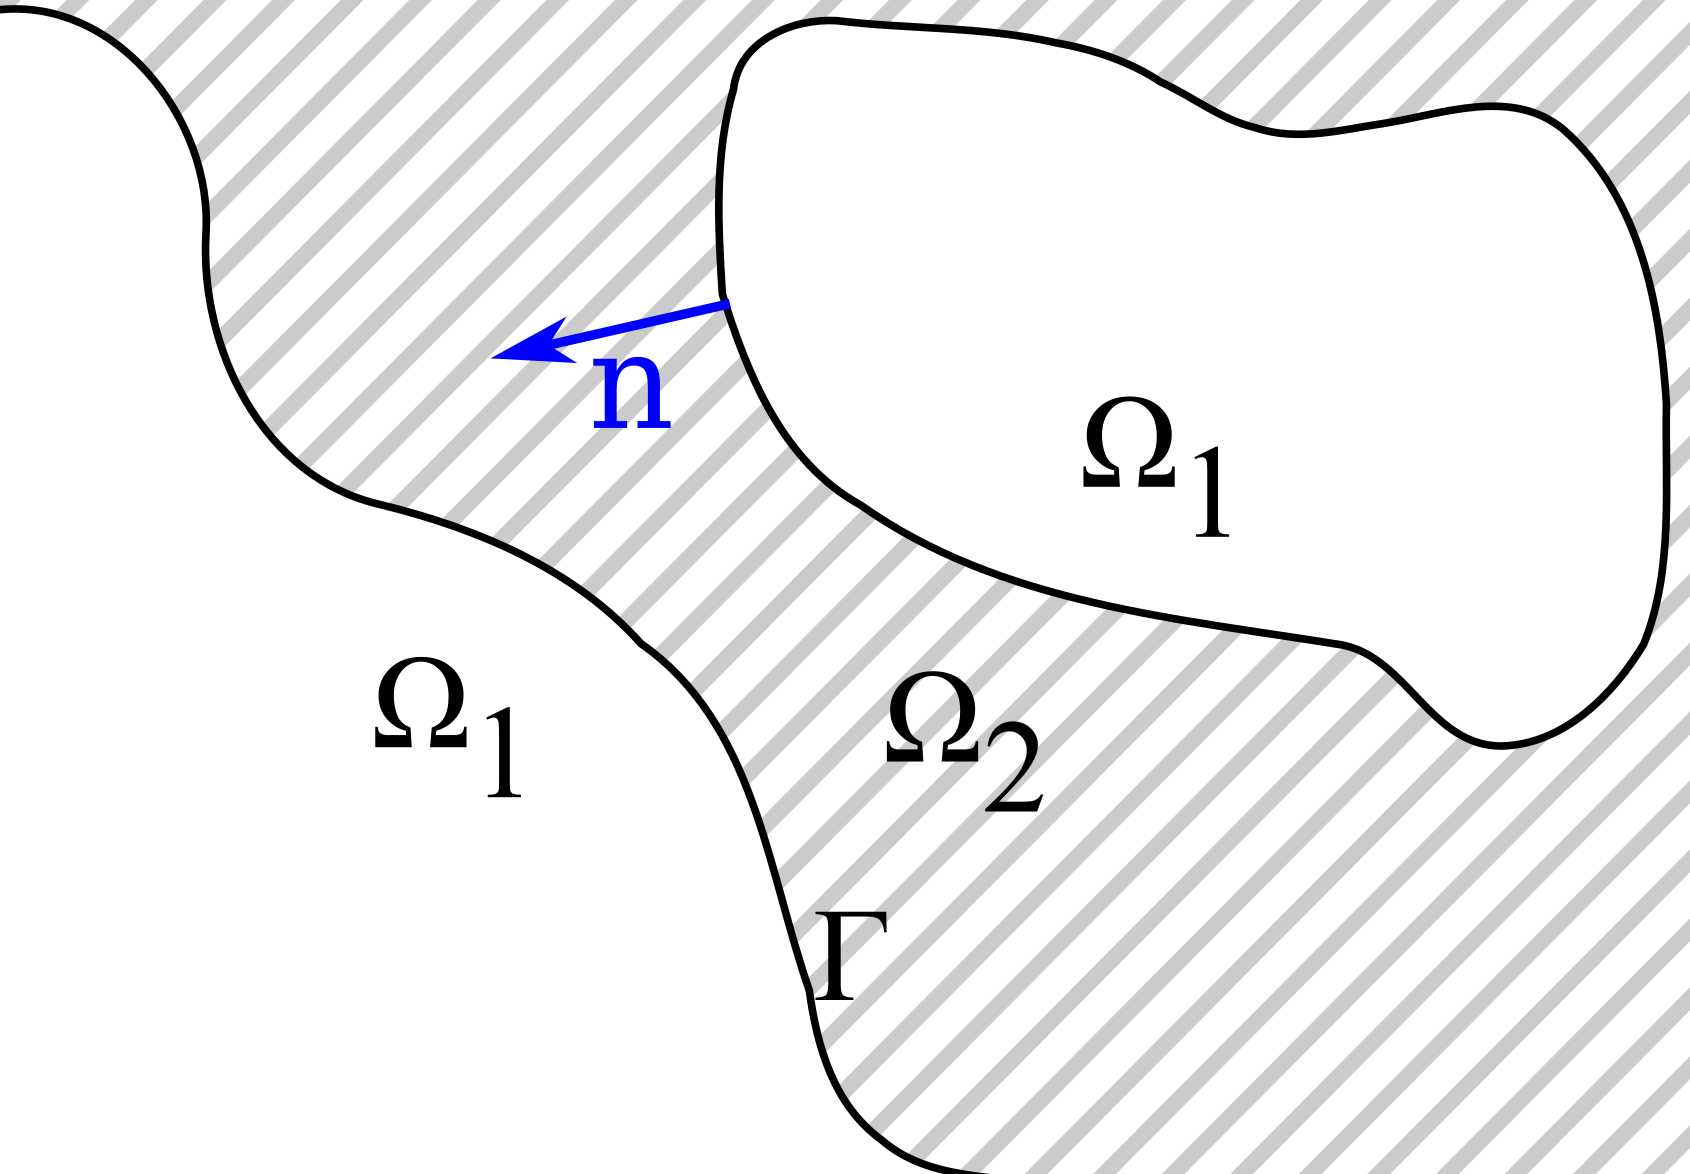
\includegraphics[width=9cm,natwidth=1690,natheight=1174]{skizze.png}\hspace*{\fill}
	\caption{Two fluid domains $\Omega_i$ separated by an interface $\Gamma$. $\vec n$ denotes the surface normal.}
	\label{intro_phases}
\end{figure}

\vspace{1cm}
The change of momentum within each fluid can be expressed as
\begin{align}
  \nabla \cdot  \vec u_i &= 0 \text{  in } \Omega_i \text{,}
	\label{nse1} \\
	\frac{\partial \vec u_i}{\partial t} + \left(\vec  u_i\cdot \nabla \right) \vec u_i
  &=
	-\frac{1}{\varrho_i}\nabla p_i + \nu_i \nabla^2 \vec u_i \text{  in } \Omega_i \text{.}
	\label{nse2}
\end{align}
Here, $\vec u_i$ is the velocity, $p_i$ the pressure, $\nu_i$ the kinematic viscosity and $\varrho_i$ the mass density.

As boundary conditions and initial conditions we use,
\begin{align}
  \vec u_i(x,t) &= 0 \text{, on } \delta\Omega_i \backslash \Gamma \text{,} \\
  \vec u_i(x,0) &= \vec u_{0,i}(x) \text{, in } \Omega_i \text{.}
\end{align}
At the interface $\Gamma$ we have a no-slip condition, i.e. continuity of the velocities between the fluid phases and the balance of viscous shear stress with surface tension. Therefore, we get the jump conditions,
\begin{align}
  [\vec u] &= 0 \text{,  } \\
  [2\mu S - p \mathbf{I}] \cdot \vec n &= 2 \sigma \kappa \vec n \text{.}
	\label{jumpconditions}
\end{align}
Here, $S$ is the shear rate tensor $S=\frac12 \left( \nabla \vec u + \nabla {\vec u}^T\right)$, $\sigma$ the surface tension, $\mu = \varrho \nu$ the dynamic viscosity and $\kappa$ the curvature of the interface with respect to its outer normal $\vec n$. Brackets denote the jump of a quantity at the interface, 
\begin{equation}
	[q](\vec x) = \lim_{\epsilon \rightarrow 0} (q(\vec x - \epsilon \vec n) - (q(\vec x + \epsilon \vec n)) \text{ with } \vec x \in \Gamma. % I also turned this around, according to [p].
\end{equation}
In \cref{intro_phases} this is the jump from $\Omega_1$ to $\Omega_2$. For the other direction the sign changes.

This paper is organized as follows: Section 2 gives an introduction to the LBM and the level set method and explains the coupling of these. In section 3 we present our results and finally in section 4 we draw a conclusion.

\section{Numerical Methods}
The algorithm we describe in this paper uses the Lattice Boltzmann Method (LBM) and the level set method. The LBM covers the description of the velocity and density field for each fluid, as it can be shown to reproduce the Navier-Stokes-equations in the asymptotic limit with Chapman-Enskog expansion \cite{LBM3}. The level set method uses a velocity field to model the movement of the interface. We will shortly introduce both methods and show how they can be coupled.

\subsection{The Lattice Boltzmann Method}
To solve the incompressible Navier-Stokes equations, we use the lattice Boltzmann method. This method describes the evolution of the particle density $f(\vec{x},\vec{v},t)$ of the Boltzmann equation in phase space, with $(\vec{x},\vec{v})$ as the phase space variables over time. For the LBM algorithm the geometrical domain is discretized with a cartesian grid and the velocity space with a restricted number of velocities adapted to this grid \cite{LBM1,LBM2,LBM3,LBM4}. We use the D2Q9 model in 2D, which has 9 velocity vectors on a plane grid with unit spacing including one zero velocity (\cref{lbmc_i}). 

\begin{figure}[h]
	\hfill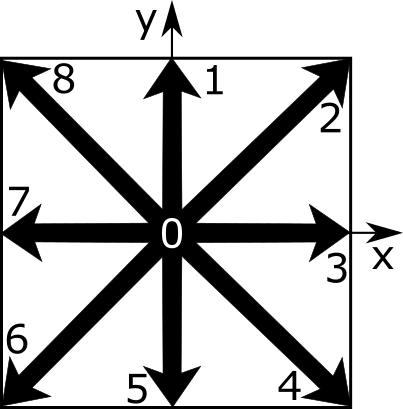
\includegraphics[trim = 0mm 0cm 0mm 35mm, clip, width=4cm,natwidth=403,natheight=409]{LBMc_i.png}\hspace*{\fill}
	\caption{The vectors of one cell in LBM.}
	\label{lbmc_i}
\end{figure}
The vectors are given by the columns of the matrix,
\begin{equation}
	c = 
	\begin{bmatrix}
	0 & 0 & 1 & 1 &  1 &  0 & -1 & -1 & -1 \\
	0 & 1 & 1 & 0 & -1 & -1 & -1 &  0 &  1
	\end{bmatrix}
	\text{.}
  \label{disc_vel}
\end{equation}
The corresponding particle distributions are denoted by $f_i(\vec{x},t) = f(\vec{x},\vec{c_i},t)$. We get the density and velocity from the moments of the particle distribution functions with,
\begin{equation}
	\rho(\vec{x},t) = \sum_{i=1}^{9} f_i(\vec{x},t) \text{, } \quad
	\vec{u} = \sum_{i=1}^{9} f_i(\vec{x},t)\vec{c_i} \text{,}
\end{equation} 
while the pressure is related to the lattice density $\rho$ as $p=\varrho \cdot \rho/3$.

The LBM algorithm alternates between a collision step and propagation step, where for the collision step we use the Bhatnagar-Gross-Krook (BGK) collision operator \cite{BGK},
\begin{equation}
	f_i^+(\vec{x}+\vec{c_i},t+1) = f_i(\vec{x},t) - \frac1\tau(f_i-f_i^{eq}) + G_i \text{.}
\end{equation}
The parameter $\tau$ is the relaxation parameter for the collision and controls the kinematic viscosity in lattice units $\nu = \frac16(2\tau - 1)$. Note, that we assume the cell spacing $\Delta x$ and the time step $\Delta t$ to be unity here. The lattice speed of sound equals to $c_s =\frac{1}{\sqrt{3}}$. $G_i$ is an additional force, e.g. gravity. In our case we set $G_i = 0$. Furthermore, we use the equilibrium distribution,
\begin{equation}
	f_i^{eq}(\rho,\vec{u}) = f_i^*(\rho + 3\vec c_i \cdot \vec{u} + \frac92(\vec c_i  \cdot \vec{u})^2 - \frac32 \vec u\cdot \vec u)
  \label{equil}
\end{equation}
with the corresponding D2Q9 weight factors,
$$
f_i^* = \begin{cases} \frac49 \text{,} & i = 0 \\ \frac19 \text{,} & i = 1,3,5,7 \\ \frac{1}{36} \text{,} &  i = 2,4,6,8 \end{cases} \text{.}
$$
The propagation step is denoted by,
\begin{equation}
	f_i(\vec{x}+\vec c_i,t+1) = f_i^+(\vec{x},t+1),
\end{equation}
%Boundary Conditions: Bounce-back & moving no-slip & inflow-outflow
where two types of boundary conditions are used. To simulate static walls we use bounce-back boundary conditions,
\begin{equation}
	\tilde{f_i} = f_{i^*}^+(\vec{x_b},t) \text{, with } \vec{x_b} \in \delta\Omega \text{,}
\end{equation}
where $i^*$ is the index of the opposite direction $\vec c_{i^*} = -\vec c_i$. To simulate a solid boundary with nonzero tangential velocity, we use moving no-slip boundary conditions,
\begin{equation}
	\tilde{f_i} = f_{i^*}^+(\vec x_b,t) + 6 f_i^*\vec c_i \vec{v} \text{, with } \vec x_b  \in \delta\Omega,
\end{equation}
where $\vec{v}$ is the speed of the moving wall. To model infinitely long domains we use periodic boundary conditions,
\begin{equation}
	\tilde{f_i}(\vec x_a ,t) = f_i^+(\vec x_b ,t) \text{,}
\end{equation}
where $x_a$ and $x_b$ are points of opposite boundaries.

One time step in the LBM algorithm is achieved by the following sub-steps:
\begin{itemize}
	\item[1. ] Collision step: $f_i^+ = f_i - \frac1\tau(f_i - f_i ^{eq}) + G_i$
	\item[2. ] Propagation step: $f_i(\vec{x}+\vec c_i ,t+1) = f_i^+(x,t)$, for $\vec{x} \in \Omega$
	\item[3. ] Boundary treatment: $f_i(\vec{x}+\vec c_i ,t+1) = f_i(\vec{x}+\vec c_i ,t)$, if $\vec{x} \notin \Omega$
\end{itemize}

We remark that the propagation step is the only non-local operation in the LBM algorithm, as it accesses nearest neighbors. This allows for highly efficient parallel implementations of the LBM.
\subsection{The Level Set Method}
We deal with the advection of the interface between the two fluids by using the level set method. The method captures the surface that represents the interface with a continuous signed distance function, where the interface is implicitly given as the zero level set.

Let $\Gamma_t$ be our interface at time t. Within the level set method, $\Gamma_t$ is the zero isosurface of the level set function $\varphi$. Thus, for $\vec x \in \Gamma_t$ we have $\varphi(\vec x,t) = 0$, in direction of the surface normal we get $\varphi > 0$, and in the other direction we get $\varphi < 0$. For this level set function we get the level set equation introduced by Osher and Sethian in \cite{OsherSethian} for the evolution of surfaces,
\begin{equation}
  \frac{\partial \varphi}{\partial t} + \vec v \cdot \nabla \varphi = 0 \text{,}
\end{equation}
with the velocity $\vec v = \vec u(\vec x(t))$ for $\vec x(t) \in \Gamma_t$, which we obtain from the LBM. It is easily visible that the normal of the surface is determined as $\vec n(x) = \frac{\nabla \varphi(x)}{\|\varphi(x)\|}$ and accordingly the curvature as the divergence of the normal $\kappa = \nabla \cdot \nabla \varphi = \Delta \varphi$.

To solve this equation we use the Toolbox of Ian Mitchell \cite{mitchell} for Matlab. This toolbox takes as input the velocity field we get from the lattice Boltzmann method and computes the movement of the interface. The toolbox also provides functions to compute the normal and the curvature of the surface. We will need this information for the coupling of the methods.

\subsection{Coupling of LBM and level set method}
The lattice Boltzmann method requires a boundary treatment at the interface which implements the macroscopic jump conditions (\ref{jumpconditions}). For the sake of simplicity, we do not write arrows for every vector, i.e., $\vec{u} \rightarrow u$. One should consider that every position, direction, and velocity is two-dimensional. 

For the coupling, we use a bounce back type boundary condition that prescribes the velocity as Dirichlet value as described in \cite[p. 1146]{Thoemmes}. Consider a point $x_2 \in \Omega_2$ that is next to the phase interface, where the link $c_i$ crosses the interface, see \cref{coupling}. We set,
\begin{figure}[h!]
	\hfill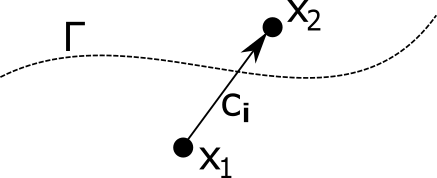
\includegraphics[width=8cm,natwidth=437,natheight=178]{coupling.png}\hspace*{\fill}
	\caption{Link between two points in different fluids.}
	\label{coupling}
\end{figure}
\begin{equation}
	f_i(x_2,t+1) = f_{i*}^+(x_2,t) + 6f_i^*c_i \cdot \tilde{u} + R_i \text{.}
\end{equation}
Here, $\tilde{u}$ describes the linear interpolation of the velocity along the direction $c_i$, evaluated at the location $\tilde{x} = x_1 + qc_i = x_2 + (q-1)c_i$ on the interface,
$$
\tilde{u} = qu(x_2,t) + (1-q)u(x_1,t) \text{.}
$$
The additional term $R_i$ ensures the jump conditions of the normal stress and corrects the error that is introduced by the first order accurate bounce back treatment above,
\begin{equation}
  R_i = 6f_i^* \left(q(q-1)\Lambda_i:[S] - (q-\frac12)\Lambda_i:S_2 \right) \text{,}
  \label{R_i}
\end{equation}
with
\begin{equation}
  \Lambda_i = c_i \otimes c_i - \frac12 (c_i \cdot c_i) \mathbf{I} \text{. }
\end{equation}
That is, an orthogonal projection of the column vectors of the (symmetric) deviatoric shear rate jump tensor on the link direction. This projection is weighted with the interface distance and a compensation term for the interpolation error. This error arises, when the interface is not on the exact center between two LBM grid cells. The tensor product is $a \otimes b = ab^T$ and the double contraction $A:B = \mathrm{trace}(AB^T)$. Furthermore, we use the following first-order estimate to obtain the shear rate from the non-equilibrium parts of the distributions, see also \cite{Krueger},
\begin{equation}
  S_k = -\frac{3}{2\tau } \sum_{i=1}^9 c_i \otimes c_i(f_i-f_i^{eq})(t,x_k) \text{.}
\end{equation}
Now we have,
\begin{equation}
  \Lambda_i:[S] = ([S]:n \otimes n)((n \cdot c_i)^2 - \frac12 (c_i \cdot c_i)) + 2([S]:n \otimes t)(n \cdot c_i)(t \cdot c_i) \text{,}
  \label{Lambda_iTimes_S}
\end{equation}
which is obtained by a coordinate transformation of (\ref{R_i}) onto a basis $(n, t)$ of normal and tangential vector to the interface. From the fluid mechanical jump condition (\ref{jumpconditions}) and the general relation $[\mu S] = \bar{\mu}[S] + [\mu]\bar{S} $ it can be seen,
\begin{align}
  [S]:n \otimes n &=  \frac{1}{2 \bar\mu} ([p] + 2 \sigma \kappa) - \frac{[\mu]}{\bar{\mu}} \bar{S} : n \otimes n \text{,} \\
  [S]:n \otimes t &= - \frac{[\mu]}{\bar{\mu}} \bar{S} : n \otimes t \text{.}
\end{align}
Here $\bar{\mu} = (\mu_1 + \mu_2)/2$ and $\bar{S} = (S_1 + S_2)/2$ are averaged quantities, $\kappa$ the interface curvature, and  $[\mu] = \mu_2 - \mu_1$ the viscosity jump.

With respect to the given definition of the discrete lattice velocities (\ref{disc_vel}, see also \cite{Thoemmes2}), the pressure jump is approximated by,
\begin{equation}
	[p] \approx \frac{1}{3} (\rho(x_2,t)\varrho_2 - \rho(x_1,t)\varrho_1) \text{.}
\end{equation}
and thus, all variables for the boundary conditions are defined. 

A refill method is still missing. Due to the fact that the interface moves, some cells change their fluid type. We use an equilibrium/non-equilibrium refill as it is described in \cite{Caiazzo} consisting of the following four steps:
\begin{itemize}
	\item[1] Extrapolate density and velocity from interior neighbors.
	\item[2] Compute the corresponding equilibrium.
	\item[3] Copy the non-equilibrium part from a direct interior neighbor.
	\item[4] Reinitialize by adding equilibrium and non-equilibrium parts.
\end{itemize}
Suppose we choose an inward pointing direction $c_i$ in a boundary point $x \in \Omega_1$, e.g. the direction with the largest angle to the surface normal. Then the density is extrapolated by,
\begin{equation}
  \tilde{\rho}(x) = 3\rho(x+c_i,t) - 3\rho(x+2c_i,t) + \rho(x+3c_i,t).
\end{equation}
\begin{figure}[h]
	\hfill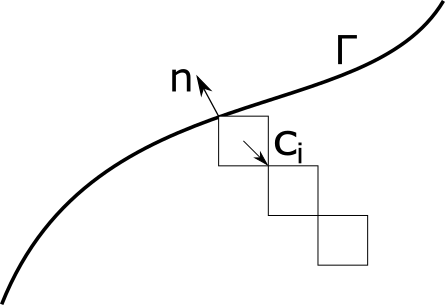
\includegraphics[width=6cm,natwidth=445,natheight=305]{refillmethod.png}\hspace*{\fill}
	\caption{Cells that are used for the refill method.}
	\label{refill}
\end{figure}
Figure \ref{refill} shows the cells we use for the extrapolation. In \cite{Thoemmes} the velocity is extrapolated using the extension velocity of the interface \cite{Adalsteinsson}. In contrast, we use the formula given in \cite{Lallemand}, analogous to the formula for the density,
\begin{equation}
  \tilde{u}(x) = 3u(x+c_i,t) - 3u(x+2c_i,t) + u(x+3c_i,t),
\end{equation}
which yields similar results, as reported in \cite{Lallemand}.
We can now compute the equilibrium part $f_i^{eq}(\tilde{\rho},\tilde{u})$ according to \cref{equil} and add it to the non-equilibrium part which we copy from a nearest neighbor,
$$f_i(\vec{x},t+1) = f_i^{eq}(\tilde{\rho},\tilde{u}) + f_i^{neq}(x+c_i,t) \text{.}$$
This completes the refill algorithm.

Finally, the complete coupling of the lattice Boltzmann and the level set method reads (see also \cref{dataexchange}):
\begin{itemize}
	\item[1.] Create the initial interface $\Gamma_0$.
	\item[2.] Run the level set code once to create the surface description for LBM.
	\item[3.] Run the LBM  for a prescribed time interval, using normal, curvature and interface position from the level set
	\item[4.] Pass the velocity field to the level set code and run it for the same time interval
	\item[5.] Repeat step 3 and 4 until the end of the simulation.
\end{itemize}
\begin{figure}[h!]
	\hfill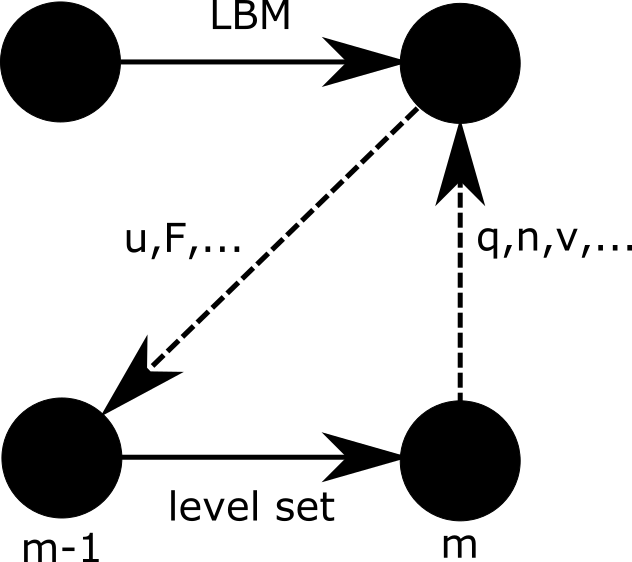
\includegraphics[width=6cm,natwidth=632,natheight=562]{dataexchange.png}\hspace*{\fill}
	\caption{Data exchange between LBM and level set method.}
	\label{dataexchange}
\end{figure}

\section{Results and Examples}
To verify the correctness of our implementation we first built a Couette flow with two stacked fluid layers. Secondly, we used the Young-Laplace experiment for a bubble to validate the implementation of surface tension.

\subsection{Couette channel flow}
\begin{figure}[h!]
	\flushright
	\hfill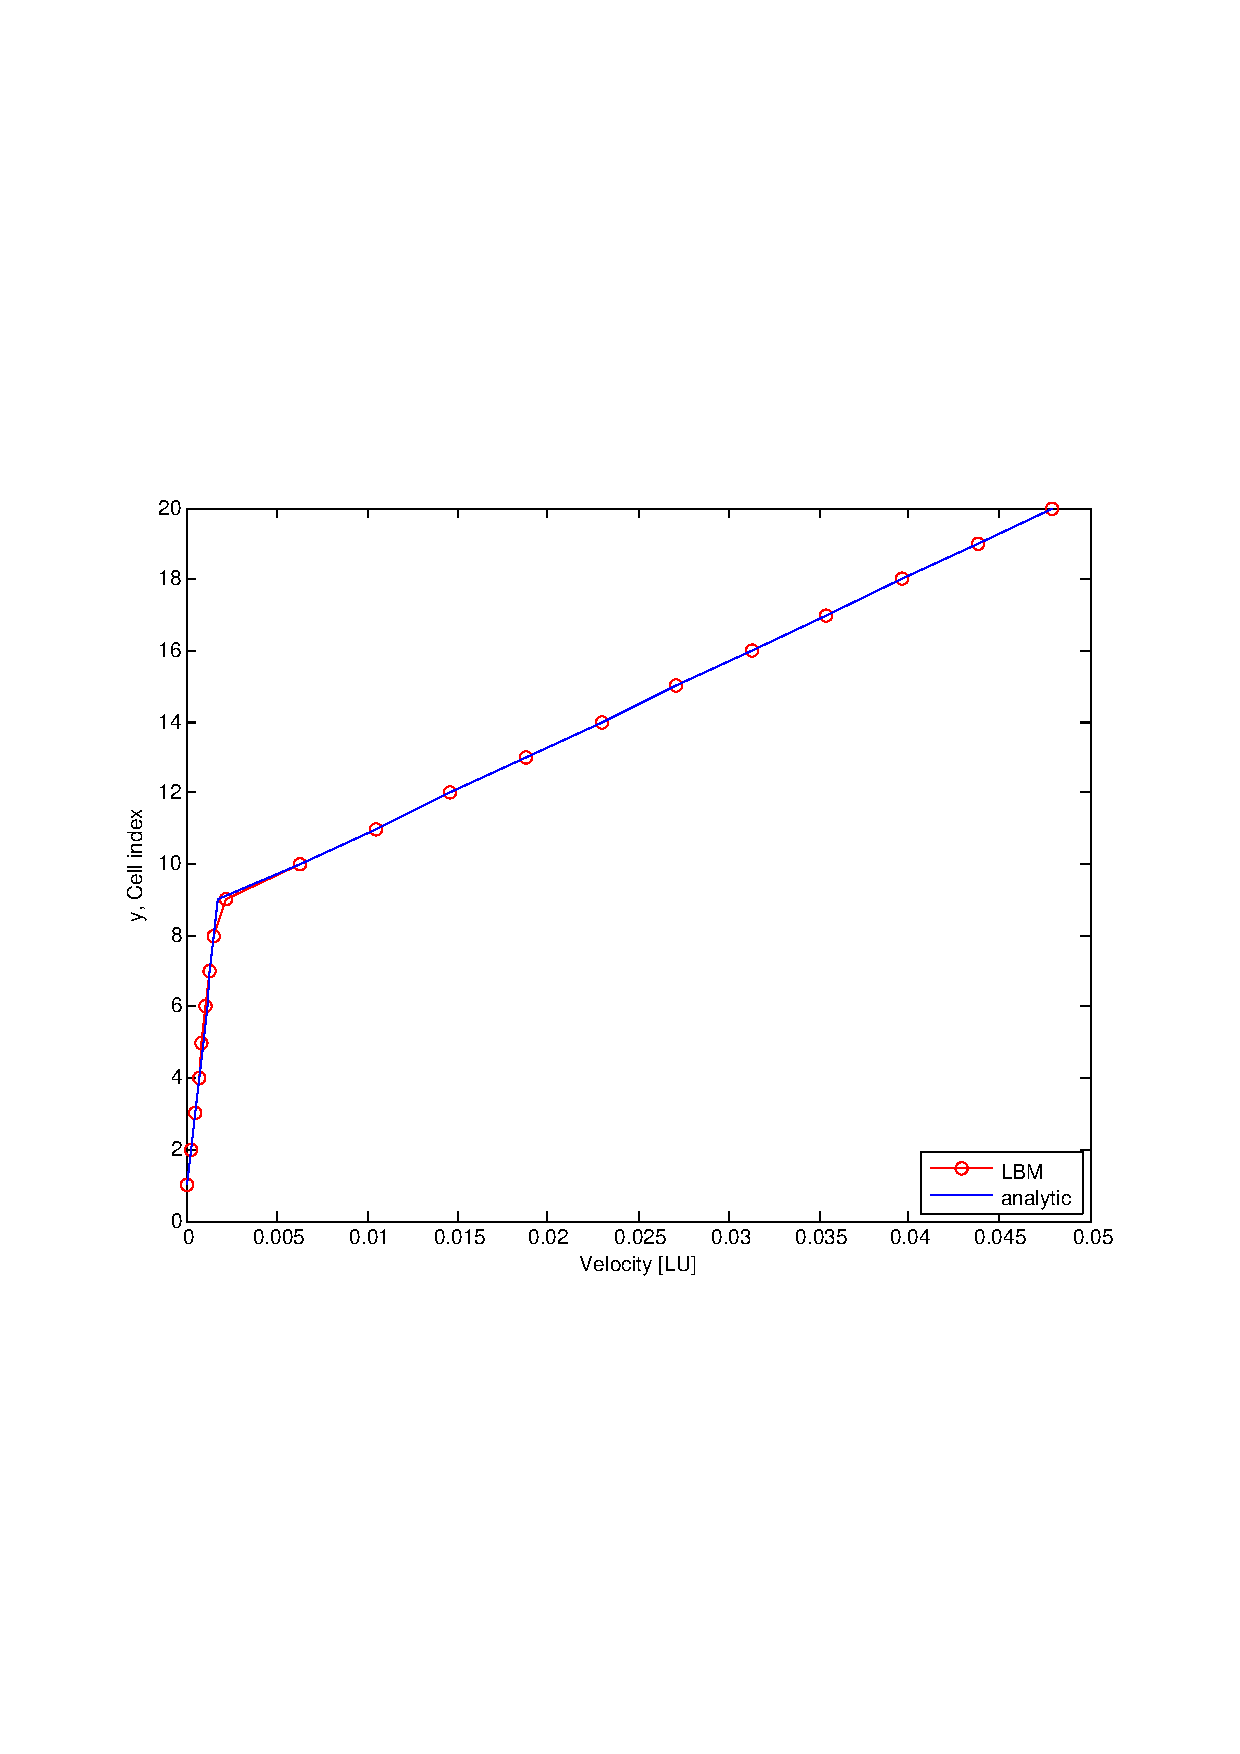
\includegraphics[trim = 0mm 8cm 0mm 8cm, clip, width=.8\textwidth, natwidth=595,natheight=842]{couette1.pdf}\hspace*{\fill}
  \caption{Two horizontal fluid layers $\Omega_i$ separated by an interface. The top boundary is moving horizontally, while the lower one is at rest}
	\label{couette1}
\end{figure}
The Couette channel flow consists of a lower wall $y=0$ at rest and an upper wall $y=1$ that is moving tangentially with a prescribed constant velocity. At these walls no-slip boundary conditions hold. Along the $x$-direction periodic boundary conditions are prescribed. The two fluids layers are oriented such that their interface is parallel to the no-slip walls, and no external pressure gradient is applied.
For this flow scenario an analytic solution can be derived from the Navier-Stokes equations, namely they simplify to $\frac{\partial }{\partial y}\left( \eta\frac{\partial u}{\partial y}\right) =0$. In combination with the no-slip conditions at top and bottom wall this means that the horizontal velocity has a linear profile with a kink at the fluid interface. The respective slopes between both phases are related by $\frac{\partial_y u^{(1)}}{\partial_y u^{(2)}} = \frac{\eta^{(2)}}{\eta^{(1)}}$.

We used identic densities $\varrho_1 = \varrho_2 = 1$ and $5 \times 20$ cells along $x \times y$ direction, as well as a LBM timestep of $\Delta t=0.0025$. In \cref{couette1} we show the simulated values and the analytic solution for viscosities $\mu^{(1)} = 1/2$ and $\mu^{(2)} = 10$, where interface was located at $y=0.42$. One can see that the values agree very well and in fact an overall relative error below $0.01\%$ was attained after 1000 LBM iterations.

Figure \ref{couette2} shows a second scenario with $5 \times 10$ cells along $x \times y$ direction and viscosities $\mu^{(1)} = 1$ and $\mu^{(2)} = 0.2$ with the interface located at $y=0.75$. Again the numerically approximated values agree very well with the analytic ones and the simulation converged at a relative error of $1.4\cdot10^{-4}$ after 2000 LBM iterations.
\begin{figure}[t!]
	\flushright
	\hfill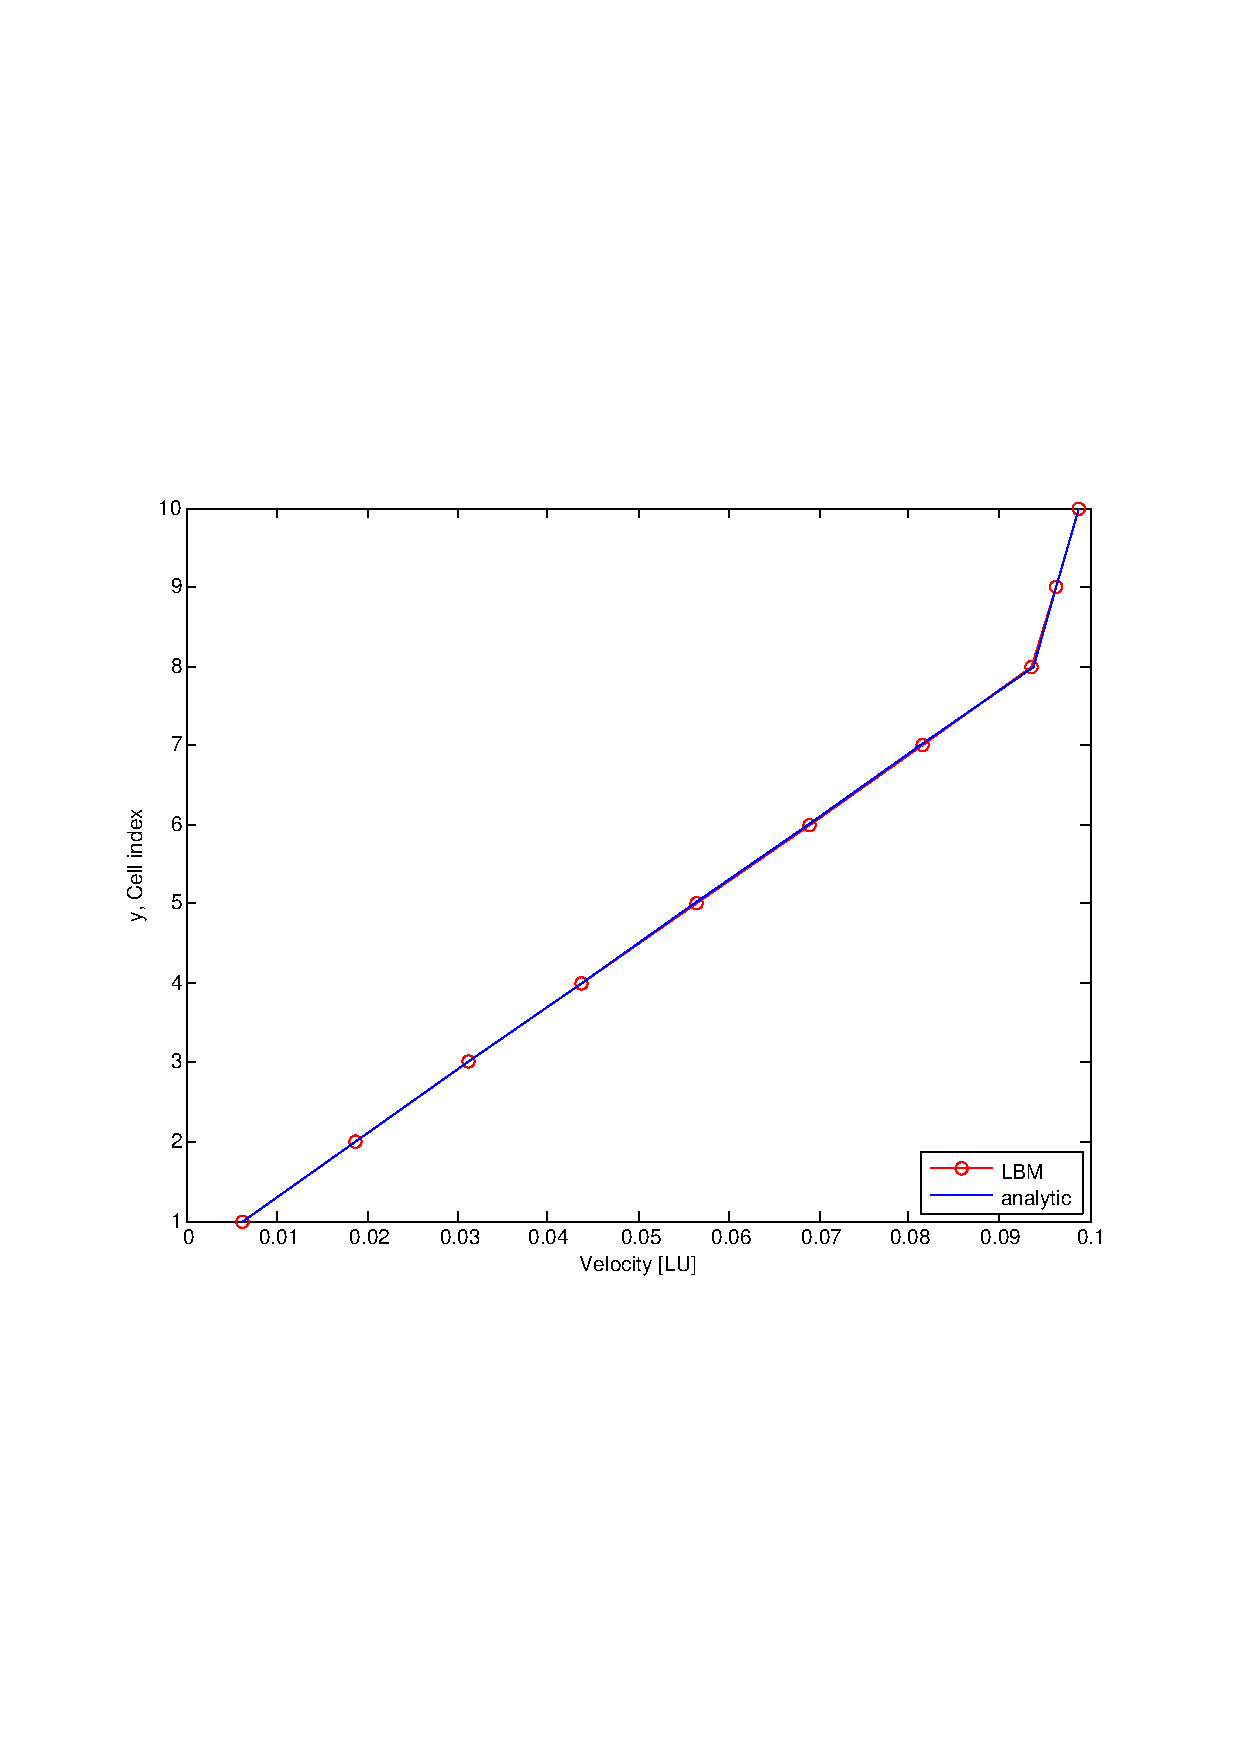
\includegraphics[trim = 0mm 8cm 0mm 8cm, clip, width=.8\textwidth, natwidth=595,natheight=842]{couette2.pdf}\hspace*{\fill}
	\caption{Two fluid domains $\Omega_i$ in a Coutte flow}
	\label{couette2}
\end{figure}
We conclude from this that the implemented LBM boundary conditions successfully model viscosity jumps at the fluid interface. Furthermore, we were able to use viscosity ratios greater than $100:1$ in our tests.
\subsection{Young-Laplace experiment for a bubble}
The Couette flow scenario does not account for the influence of surface tension as the fluid interface is not curved. If it would get distorted, surface tension would have a stabilizing effect although. 
Hence, we use the Young-Laplace law for the pressure drop across curved surfaces to validate the implementation of surface tension. Due to surface tension the pressure inside of convex surfaces is generally higher than on the outside and the pressure drop $\Delta p$ of a bubble of radius $r$ is proportional to the surface tension coefficient $\sigma$ according to the following relationship,
\begin{equation}
	\Delta p = \frac{2\sigma}{r} = 2 \sigma \kappa .
\end{equation}

Figure \ref{laplace} shows the simulation results we obtained for a $40 \times 40$ cells grid over a $[0,1]\times[0,1]$-domain with periodic boundaries. At the center, a sphere of radius $0.25$ was placed with $\varrho_2 = 1.1$ while the exterior contained a fluid with $\varrho_1 = 1$. It is visible, how the approximated pressure attains the analytical solution in a oscillatory motion with decaying amplitude, until both values agree. The algorithm needed 1000 LBM-iterations, where every ten iterations a call to the level-set routine was executed. Both fluids had an identical viscosity of $\nu = 1/6$.
\begin{figure}[t!]
	\flushright
	\hfill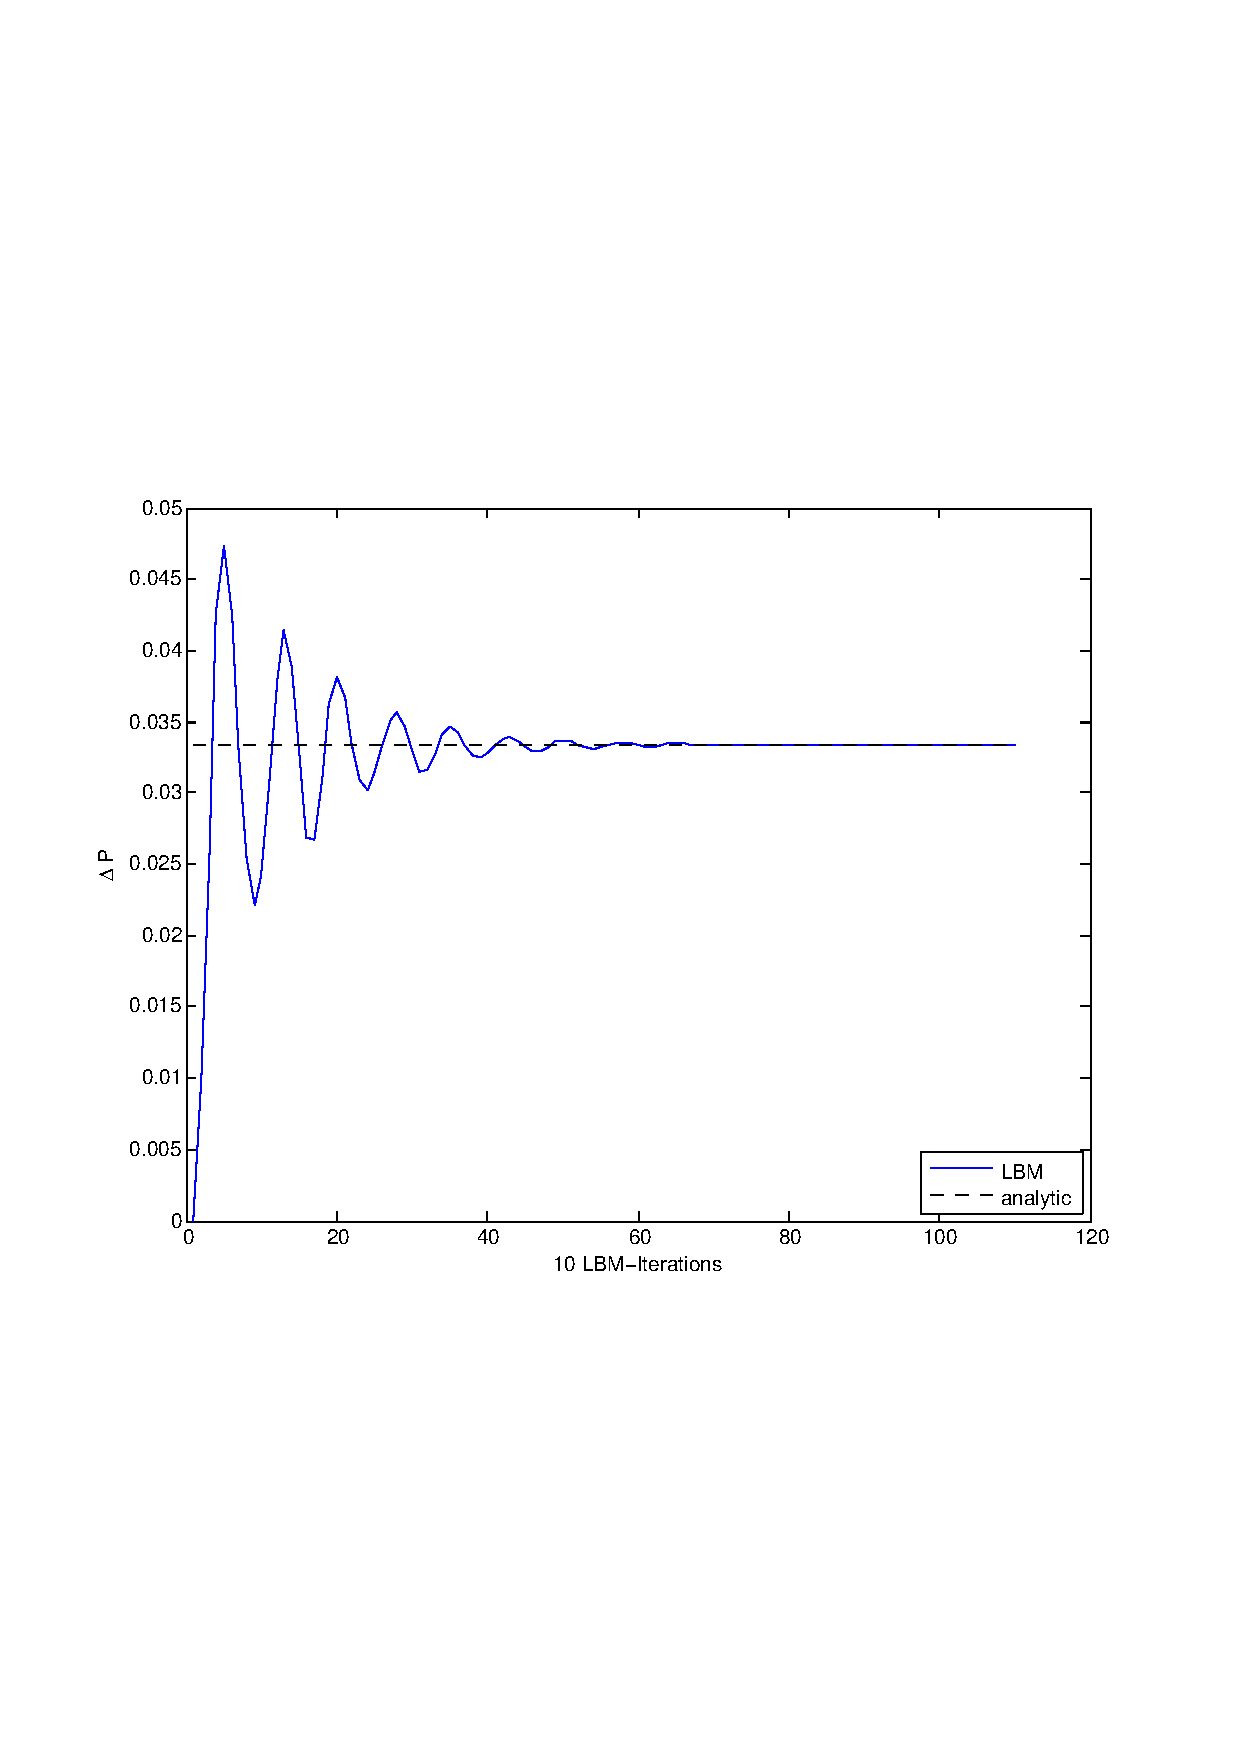
\includegraphics[trim = 0mm 7.75cm 0mm 8.06cm, clip, width=.8\textwidth, natwidth=595,natheight=842]{laplace.pdf}\hspace*{\fill}
	\caption{The pressure drop of a spherical bubble over LBM iterations}
	\label{laplace}
\end{figure}
We noted that the velocity close to the interface contained erroneous components, which lead to a slight distortion of the spherical shape. We explain those fluxes as inaccuracies stemming from the used level set subroutines, according to the analysis shown in \cite{Thoemmes2}.
Additionally, we want to state that we were not able to attain stable results for surface tension coefficients $\sigma > \mathrm{O(10^{-3})}$. Large densitiy ratios were limited to big viscosity regimes or refined spatial resolution in our tests.

\section{Conclusion}
We implemented a hybrid lattice Boltzmann method that uses the level set method to model the movement of the interface. The implementation was done in Matlab for a two dimensional case. We adapted the formulas given in \cite{Thoemmes} to fit in our environment. Finally, we verified our implementation with different test cases.

A more vivid possible application of the algorithm we presented is shown in \cref{cavity}, which shows the transient movement of an oil drop in a lid driven cavity. It is a known problem that level set methods tend to suffer from mass losses \cite{Thoemmes}, but still a very good insight into the detailed flow behavior is possible. Accordingly, a variety of two-phase flow scenarios is possible for simulation with the presented method.

The authors want to thank Ian Mitchell for providing the toolbox for level set methods.
\begin{figure}
	\hfill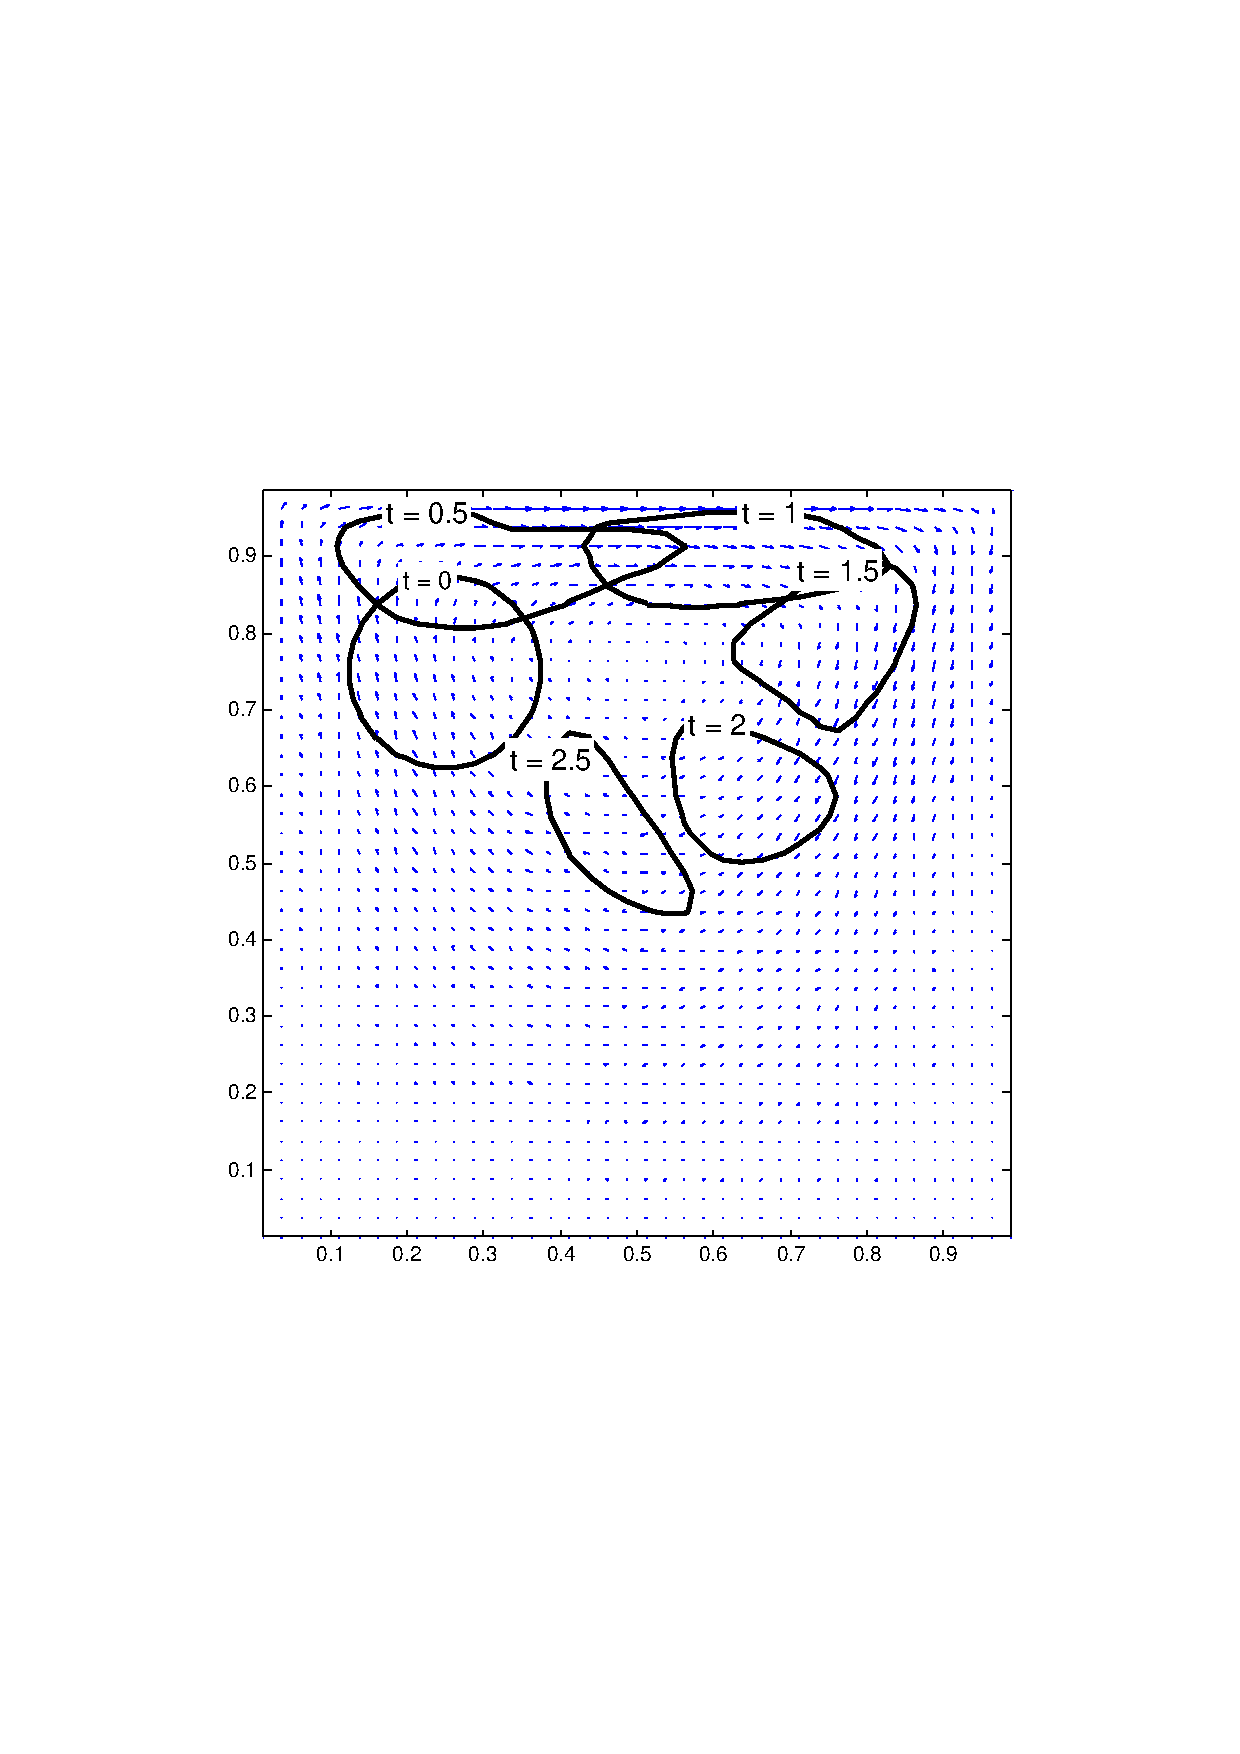
\includegraphics[trim = 0mm 8cm 0mm 8.0cm, clip, width=.95\textwidth, natwidth=595,natheight=842]{cavity.pdf}\hspace*{\fill}
	\caption{The transient flow and deformation of a bubble in a lid driven cavity. The black lines show the interface at different points of time and the arrows display the velocity field.}
	\label{cavity}
\end{figure}

\begin{thebibliography}{1}	

\bibitem{Thoemmes} {\sc G. TH\"OMMES, J. BECKER, M. JuNK, A.K. VAIKUNTAM, D. KEHRWALD, A. KLAR, K. STEINER, A. WIEGMANN}, A lattice Boltzmann method for immiscible multiphase flow simulations using the level set method, J. Comput. Phys. 228 (2009), 1139-1156.

\bibitem{Thoemmes2} {\sc J. BECKER, M. JUNK, D. KEHRWALD, G. TH\"OMMES, Z. YANG}, A combined lattice BGK/level set method for immiscible two-phase flows, Computers and Mathematics with Applications, 58(5):950–964, 2009.

\bibitem{ferziger} {\sc J. FERZIGER, M. PERIC.}, Computational methods for fluid dynamics. Springer Science \& Business Media, ISBN 978-3540420743 (2012).

\bibitem{Adalsteinsson} {\sc D. ADALSTEINSSON, J.A. SETHIAN}, The fast construction of extension velocities in level set methods, J. Comput. Phys. 148 (2) (1999) 2–22.

\bibitem{trygg} {\sc G. TRYGGVASON, R. SCARDOVELLI, S. ZALESKI}, Direct Numerical Simulations of Gas-Liquid Multiphase Flows, Cambridge University Press, ISBN 9780521782401 (2011)

\bibitem{GRcg1} {\sc A.K. GUNSTENSEN, D.H. ROTHMAN, S. ZALESKI, G. ZANETTI}, Lattice Boltzmann model of immiscible fluids, Phys. Rev. A 43 (8) (1991) 4320-4327.

\bibitem{GRcg2} {\sc A.K. GUNSTENSEN, D.H. ROTHMAN}, Macroscopic modeling of immiscible flows in three dimensions by a lattice Boltzmann method, Europhys. Lett. 18 (2) (1998) 157-161.
	
\bibitem{GRcg3} {\sc K. SANKARANARAYANAN, I.G. KEVREKIDIES, S. SUNDARESAN, J. LU, G. TRYGGVASON}, A comparative study of lattice Boltzmann and front-tracking finite-difference methods for bubble simulations, Int. J. Multiphase Flow 29 (1) (2003) 109-116.

\bibitem{ShanChen1} {\sc X. SHAN, H. CHEN}, Lattice Boltzmann model for simulation flows with multiple phases and components, Phys. Rev. E 47 (3) (1999) 567-603.

\bibitem{ShanChen2} {\sc X. SHAN, H. CHEN}, Simulation of nonideal gases and liquid-gas phase transition by the Lattice Boltzmann equation, Phys. Rev. E 49 (4) (1994) 2941.
	
\bibitem{Koerner} {\sc C. K\"ORNER, M. THIES, T. HOFMANN, N. TH\"UREY, U. R\"UDE}, Lattice Boltzmann Model for Free Surface Flow for Modeling Foaming, J. Stat. Phys. 121 (2005) 179-196.

\bibitem{Scardovelli} {\sc R. SCARDOVELLI, S. ZALESKI}, Direct numerical simulation of free-surface and interfacial flow, Annu. Rev. Fluid Mech. 31 (1999) 567-603.

\bibitem{Hirt} {\sc C.W. HIRT, J.P. SHANNON}, Free-surface stress conditions for incompressible-flow calculations, J. Comput. Phys. 2 (1968) 403-411

\bibitem{LBM1} {\sc S. CHEN, G.D. DOOLENM}, Lattice Boltzmann method for fluid flows, Ann. Rev. Fluid Mech. 30 (1998) 329-364.

\bibitem{LBM2} {\sc X. HE, L.S. LUO}, Lattice Boltzmann model for the incompressible Navier-Stokes equation, J. Stat. Phys. 88 (1997) 927-944.

\bibitem{LBM3} {\sc S. SUCCI}, The Lattice Boltzmann Equation for Fluid Dynamics and Beyond, Clarendon Press, Oxford, ISBN 978-0-19-850398-9 (2001).

\bibitem{LBM4} {\sc D.A. WOLF-GLADOW}, Lattice-Gas Cellular Automata and Lattice Boltzmann Models, An Introduction, Springer, (2000).

\bibitem{BGK} {\sc P. BHATNAGAR, E. GROSS, M. KROOK}, A model for collision processes in gases: 1. Small amplitude processes in charged and neutral one-component systems, Phys. Rev. 94 (1954) 511.

\bibitem{OsherSethian} {\sc S. OSHER, J. SETHIAN}, Fronts propagating with curvature-dependent speed: algorithms based on Hamlton-Jacobi formulations, J. Comput. Phys. 79 (1988) 12-49.

\bibitem{mitchell}I. MITCHELL, A Toolbox of Level Set Methods, August 2015, URL: \url{http://www.cs.ubc.ca/~mitchell/ToolboxLS/}.

\bibitem{Caiazzo} {\sc A. CAIAZZO}, Asymptotic analysis of lattice Boltzmann method for fluid-structure interaction problems, Ph.D. Thesis, Kaiserslautern (Germany) and Pisa (Italy), 2007.

\bibitem{Krueger} {\sc T. KR\"UGER, F. VARNIK, D. RAABE}, Shear stress in lattice Boltzmann simulations, Phys. Rev. E 79 (4) (2009) 046704.

\bibitem{Lallemand} {\sc P. LALLEMAND, L.-S. LUO}, Lattice Boltzmann method for moving boundaries, J. Comput. Phys. 184 (2003) 406-421.

\end{thebibliography}


\end{document}
%% end of file `docultexmm.tex'
